\documentclass[11pt]{article}
\usepackage{mathtools,amssymb}
\usepackage{geometry,pgfplots}
\usepackage{fullpage,parskip}
\usepackage{graphicx}
\usepackage{enumitem}
\usepackage{hyperref}
\pgfplotsset{compat=1.15}

\newcommand{\sol}{\textbf{\textit{Solution: }}}
\newcommand{\solnum}[1]{\textbf{\textit{Solution #1: }}}
\newcommand{\dir}[0]{\measuredangle}

\begin{document}
\begin{center} \bfseries \large
    February Monthly Problem Set Solutions

    % Due date: 21 February 2025
\end{center}

% \bigskip
% Submit your monthly problem sets here: \url{https://forms.gle/pZH93Fq95UuABT277}.
% You can ask the coaches from the Stellenbosch Camp for hints, but do not ask other people for help or look for help online.

\begin{enumerate}[topsep=\bigskipamount,itemsep=\bigskipamount,leftmargin=0pt]
% C
\item % BJ-2018-4
$2025$ people sit around a circular table.
Every hour there is a vote, where each person votes either yes or no.
Each person $X$ obeys the following rule.
On the $n$th hour, if $X$'s vote is the same as that of at least one of the neighbours of $X$, then $X$'s vote will be the same on the $(n+1)$th hour as on the $n$th hour; otherwise, $X$'s vote on the $(n+1)$th hour will be dif and only iferent from $X$'s vote on the $n$th hour.

Prove that, irrespective of how everyone votes on the first hour, there will be an hour after which nobody's vote will ever change.

\sol % Tim
A person's vote only changes if they are in between two neighbours that disagree with them.

Consider someone who does not change at a certain hour. They will never change again: since they did not change, they have at least one neighbour who agrees with them. This neighbour then has a neighbour (the original person) who agrees with them, and neither of them will ever change.

Now, assume for contradiction that there is no hour after which everybody's vote will never change. Each person either reaches a point after which they never change, or they always change. Consider only the people that always change. There must be at least one of these.

For person $X$ to always change, both of his neighbours must always oppose him. This means that both of his neighbours must always change. Continuing this pattern, everyone must always change.

Hence, in a single round, every person must differ from both their neighbours i.e. the votes should alternate. Since 2025 is odd, this is impossible.

% N
\item % JM-2019-2
Let $f,g : \mathbb{Z} \to \mathbb{Z}$ be two functions such that $|f(x)| \leqslant |x|$ and $f(3x+4y) = g(2x+5y)$ for all $x,y \in \mathbb{Z}$.
Find the largest possible value of $f(2025)$.

\sol
Let $n \in \mathbb{Z}$; by Bezout's Lemma, there are $x,y \in \mathbb{Z}$ such that $3x+4y = n$.
Thus
\[ f(n) = f(3x+4y) = g(2x+5y) = g(2(x+5)+5(y-2)) = f(3(x+5)+4(y-2)) = f(n+7) \]
and so $f$ is periodic with period $7$.
Similarly, $g$ is also periodic with period $7$.
Thus $|f(2025)| = |f(2)| \leq 2$, so that $f(2025)$ is at most $2$.

Now to show that we can actually have $f(2025) = 2$, we can define functions $f$ and $g$ which satisfy the problem conditions as follows:
\[ f(x) = \begin{cases}
    0 & \text{if} \ x \equiv_7 0 \\
    1 & \text{if} \ x \equiv_7 \pm 1 \\
    2 & \text{if} \ x \equiv_7 \pm 2 \\
    3 & \text{if} \ x \equiv_7 \pm 3
\end{cases} \quad\text{and}\quad g(x) = \begin{cases}
    0 & \text{if} \ x \equiv_7 0 \\
    1 & \text{if} \ x \equiv_7 \pm 2 \\
    2 & \text{if} \ x \equiv_7 \pm 3 \\
    3 & \text{if} \ x \equiv_7 \pm 1
\end{cases}. \]
To see why this definition works, note that $2x+5y \equiv_7 3(3x+4y)$ for $x,y \in \mathbb{Z}$, so since $f$ and $g$ are periodic with period $7$ the given condition is equivalent to saying that $g(3x) = f(x)$ for $x \in \mathbb{Z}$.
It is not hard to see that the functions defined above satisfy this condition.

% A
\newcommand*{\parens}[1]{\left(#1\right)}
\item % LB-2019-3
Let $a$, $b$, $m$, and $n$ be positive integers such that $a \neq b$. Show that
\[ \frac{\parens{a-b}\parens{a^2-b^2}\dotsb\parens{a^{m+n}-b^{m+n}}}{\parens{a-b}\parens{a^2-b^2}\dotsb\parens{a^m-b^m} \cdot \parens{a-b}\parens{a^2-b^2}\dotsb\parens{a^n-b^n}} \]
is an integer.

\sol
Firstly, consider the case where $m=1$.
The fraction is then:
\[ \frac{\parens{a-b}\parens{a^2-b^2}\dotsb\parens{a^{1+n}-b^{1+n}}}{\parens{a-b} \cdot \parens{a-b}\parens{a^2-b^2}\dotsb\parens{a^n-b^n}} = \frac{a^{1+n}-b^{1+n}}{a-b} = a^n +a^{n-1}b +\dotsb +ab^{n-1} +b^n \in \mathbb{Z}. \]
The computation is similar if $n=1$.
We will now prove the problem by induction on $m+n$.
In the base case where $m+n = 2$, both $m=1$ and $n=1$ and so it is covered by the preceding argument.
Now suppose that the result is true if $m+n = k$ for some $k \in \mathbb{N}$, and consider now if $m+n = k+1$.
If either $m=1$ or $n=1$ then the preceding argument applies; so assume that $m,n > 2$.
Then since $a^{m+n}-b^{m+n} = a^m(a^n-b^n) +b^n(a^m-b^m)$, we have that
\begin{align*}
    &\mathrel{\phantom{=}} \frac{\parens{a-b}\parens{a^2-b^2}\dotsb\parens{a^{m+n}-b^{m+n}}}{\parens{a-b}\parens{a^2-b^2}\dotsb\parens{a^m-b^m} \cdot \parens{a-b}\parens{a^2-b^2}\dotsb\parens{a^n-b^n}} \\
    &= \begin{multlined}[t]
        a^m \times \frac{\parens{a-b}\parens{a^2-b^2}\dotsb\parens{a^{m+n-1}-b^{m+n-1}}}{\parens{a-b}\parens{a^2-b^2}\dotsb\parens{a^m-b^m} \cdot \parens{a-b}\parens{a^2-b^2}\dotsb\parens{a^{n-1}-b^{n-1}}} \\
        +b^n \times \frac{\parens{a-b}\parens{a^2-b^2}\dotsb\parens{a^{m-1+n}-b^{m-1+n}}}{\parens{a-b}\parens{a^2-b^2}\dotsb\parens{a^{m-1}-b^{m-1}} \cdot \parens{a-b}\parens{a^2-b^2}\dotsb\parens{a^n-b^n}}.
    \end{multlined}
\end{align*}
Since $(m-1)+n = m+(n-1) = k$, both of the fractions above are integers by the induction hypothesis, and so the full fraction is an integer.
Thus by induction the original statement is proved.

% G
\item % 2016 Bulgaria JBMO TST 2.2 (Adapted)
The vertices of the pentagon $ABCDE$ lie on a circle in that order.
The points $H_1$, $H_2$, $H_3$, $H_4$ are the orthocentres of the triangles $ABC$, $ABE$, $ACD$, $ADE$ respectively.
Prove that the quadrilateral determined by the four orthocentres is a rhombus 
%if and only if $BE \parallel CD$.
if and only if $BE\parallel CD$ or $BC\parallel DE$.

\solnum{1}
For any triangle $ABC$ in the complex plain with circumcentre $O$, orthocentre $H$ and centroid $G$, one has that $3(G-O) = H-O$ and $G = (A+B+C)/3$.
If $O$ is the origin, then $H = A+B+C$.

The triangles in the question share their circumcentre, say $O$.
Place this in the complex plane with $O$ as the origin.
Then
\begin{align*}
    H_1 & = A+B+C, & H_2 & = A+B+E, & H_3 & = A+C+D, & \text{and} \quad H_4 & = A+D+E,
\end{align*}
\[ \implies \quad \frac{H_1+H_4}{2} = \frac{H_2+H_3}{2}. \]
Thus $H_1H_2H_4H_3$ is a parallelogram in that order with diagonals $H_1H_4$ and $H_2H_3$.

Let $M_1$, $M_2$, $M_3$, and $M_4$ be the midpoints of $BC$, $CD$, $DE$, and $EB$ respectively.
Now $M_1M_2M_3M_4$ is a parallelogram with $M_1M_2 = BD/2$ and $M_2M_3 = CE/2$.
Also
\begin{align*}
    (H_1-H_4)/2 &= (B+C)/2 - (D+E)/2 = M_1 - M_3 \quad \text{and} \\
    (H_2-H_3)/2 &= (B+E)/2 - (C+D)/2 = M_2 - M_4.
\end{align*}
Thus $H_1H_2H_4H_3$ is a rhombus
if and only if $H_1H_4 \perp H_2H_3$
if and only if $M_1M_3 \perp M_2M_4$
if and only if $M_1M_2M_3M_4$ is a rhombus
if and only if $M_1M_2 = M_2M_3$
if and only if $BD = CE$
if and only if $BCDE$ is an isosceles trapezium (remember $BCDE$ is cyclic)
if and only if $BE \parallel CD$ or $BC\parallel DE$.

%Preliminary diagram\\
%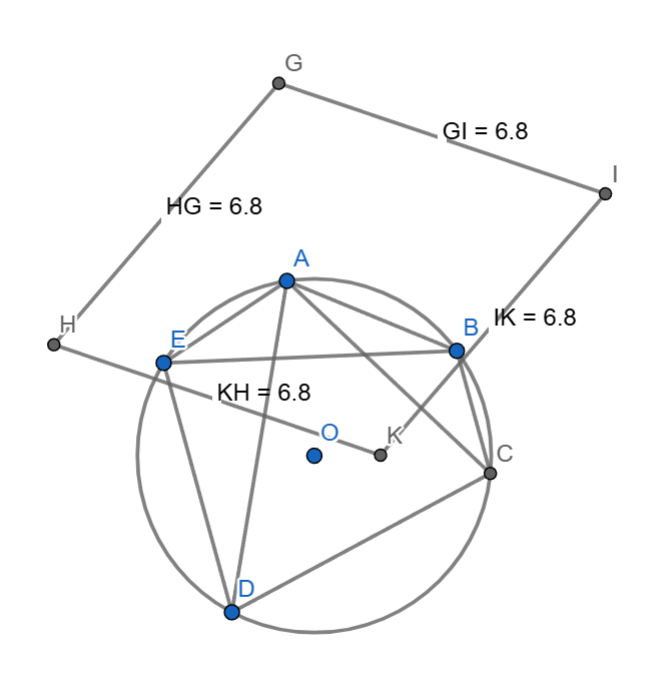
\includegraphics[scale=0.5]{Advanced/M2 Q4.png}

\solnum{2} This proof uses directed angles modulo $180^{\circ}$ ($\dir ABC$ meaning directed angle $AB$ to $BC$).

\textbf{\textit{Lemma 1:}} Given cyclic quadrilateral $ABCD$, let $H_A$ be the orthocentre of $\triangle ACD$ and $H_B$ be the orthocentre of $\triangle BCD$. Then $H_AH_B \parallel AB$ and $H_AH_B=AB$.

\textbf{\textit{Proof of Lemma:}} Let $E$, $F$, and $G$ be the feet of the perpendiculars from $C$, $D$, and $A$ to $DB$, $AC$, and $DB$ respectively.
Since $\dir DH_AC=\dir DAC=\dir DBC=\dir DH_BC$ and so $DH_AH_BC$ is cyclic.
Notice that $ADFG$ is cyclic so $\dir CAG\equiv\dir FAG = \dir FDG$.
Since $\dir CAB = \dir CDB$ ($ABCD$ is cyclic) we get $\dir GAB = \dir CDF$.
And from $DH_AH_BC$ being cyclic we can extend this to $\dir GAB = \dir CDF = \dir EH_BH_A$.
Now we have $AG\parallel H_BE\implies \dir H_BAG = \dir AH_BE$ and combined with $\dir GAB = \dir EH_BH_A$ gives $\dir H_BAB = \dir AH_BH_A\implies H_AH_B\parallel AB$.
Since $AH_A\parallel BH_B$ (both are perpendicular to $DC$) we get that $ABH_BH_A$ is a parallelogram and so $H_AH_B=AB$. $\hfill\square$

\begin{center}
\definecolor{uququq}{rgb}{0.25098039215686274,0.25098039215686274,0.25098039215686274}
\definecolor{uuuuuu}{rgb}{0.26666666666666666,0.26666666666666666,0.26666666666666666}
\definecolor{xdxdff}{rgb}{0.49019607843137253,0.49019607843137253,1}
\begin{tikzpicture}[scale=0.8,line cap=round,line join=round,x=1cm,y=1cm]
\tikzstyle{every node}=[font=\large]
\clip(-5.7452516904583,-4.467783621337356) rectangle (4.730330578512396,4.457836213373419);
\draw[line width=2pt,color=uququq,fill=uququq,fill opacity=0.1] (-0.3127707382719036,0.624128849615983) -- (-0.16295536206046377,0.47341963471879467) -- (-0.012246147163275406,0.6232350109302346) -- (-0.16206152337471527,0.773944225827423) -- cycle; 
\draw[line width=2pt,color=uququq,fill=uququq,fill opacity=0.1] (1.6772775344122512,0.020601895953523713) -- (1.7679348567264506,-0.17159374477519193) -- (1.960130497455166,-0.08093642246099253) -- (1.8694731751409668,0.11125921826772309) -- cycle; 
\draw[line width=2pt,color=uququq,fill=uququq,fill opacity=0.1] (1.7008144754960504,2.625771725535885) -- (1.5509990992846105,2.776480940433073) -- (1.4002898843874223,2.6266655642216334) -- (1.5501052605988621,2.475956349324445) -- cycle; 
\draw [shift={(0.03525497990376868,3.9998446327816266)},line width=2pt,color=uququq,fill=uququq,fill opacity=0.1] (0,0) -- (-45.17041212187076:0.6761833208114199) arc (-45.17041212187076:-18.066285072987455:0.6761833208114199) -- cycle;
\draw [shift={(0.03525497990376868,3.9998446327816266)},line width=2pt,color=uququq,fill=uququq,fill opacity=0.1] (0,0) -- (-64.74708016382165:0.45078888054094657) arc (-64.74708016382165:-45.170412121870754:0.45078888054094657) -- cycle;
\draw [shift={(3.1090598946163057,-2.5166935792202523)},line width=2pt,color=uququq,fill=uququq,fill opacity=0.1] (0,0) -- (115.25291983617835:0.6761833208114199) arc (115.25291983617835:134.82958787812927:0.6761833208114199) -- cycle;
\draw [shift={(-3.2650848468196174,-2.3106754300569596)},line width=2pt,color=uququq,fill=uququq,fill opacity=0.1] (0,0) -- (25.252919836178343:0.6761833208114199) arc (25.252919836178343:44.82958787812926:0.6761833208114199) -- cycle;
\draw [shift={(-3.2650848468196174,-2.3106754300569596)},line width=2pt,color=uququq,fill=uququq,fill opacity=0.05] (0,0) -- (-1.8512072127049428:0.8264462809917354) arc (-1.8512072127049428:25.252919836178354:0.8264462809917354) -- cycle;
\draw [shift={(-0.12076997229954275,-0.8275243764955856)},line width=2pt,color=uququq,fill=uququq,fill opacity=0.1] (0,0) -- (-154.74708016382166:0.45078888054094657) arc (-154.74708016382166:-27.609123976057:0.45078888054094657) -- cycle;
\draw [shift={(2.1740318564046013,-1.5760869131403807)},line width=2pt,color=uququq,fill=uququq,fill opacity=0.1] (0,0) -- (-172.3083683096354:0.45078888054094657) arc (-172.3083683096354:-45.170412121870726:0.45078888054094657) -- cycle;
\draw [shift={(0.03525497990376868,3.9998446327816266)},line width=2pt,color=uququq,fill=uququq,fill opacity=0.1] (0,0) -- (-117.60912397605699:0.45078888054094657) arc (-117.60912397605699:-64.74708016382165:0.45078888054094657) -- cycle;
\draw [shift={(2.330056808607913,3.251282096136831)},line width=2pt,color=uququq,fill=uququq,fill opacity=0.1] (0,0) -- (-135.17041212187075:0.45078888054094657) arc (-135.17041212187075:-82.3083683096354:0.45078888054094657) -- cycle;
\draw [shift={(2.1740318564046013,-1.5760869131403807)},line width=2pt,color=uququq,fill=uququq,fill opacity=0.1] (0,0) -- (134.82958787812925:0.7513148009015777) arc (134.82958787812925:161.93371492701255:0.7513148009015777) -- cycle;
\draw [shift={(2.1740318564046013,-1.5760869131403807)},line width=2pt,color=uququq,fill=uququq,fill opacity=0.1] (0,0) -- (110.98546581311562:0.8264462809917354) arc (110.98546581311562:134.82958787812925:0.8264462809917354) -- cycle;
\draw [shift={(0.03525497990376868,3.9998446327816266)},line width=2pt,color=uququq,fill=uququq,fill opacity=0.1] (0,0) -- (-69.01453418688439:0.8264462809917354) arc (-69.01453418688439:-45.17041212187077:0.8264462809917354) -- cycle;
\draw [line width=2pt] (0,0) circle (4cm);
\draw [line width=2pt] (0.03525497990376868,3.9998446327816266)-- (-3.2650848468196174,-2.3106754300569596);
\draw [line width=2pt] (-3.2650848468196174,-2.3106754300569596)-- (3.1090598946163057,-2.5166935792202523);
\draw [line width=2pt] (3.1090598946163057,-2.5166935792202523)-- (2.330056808607913,3.251282096136831);
\draw [line width=2pt] (2.330056808607913,3.251282096136831)-- (0.03525497990376868,3.9998446327816266);
\draw [line width=2pt] (0.03525497990376868,3.9998446327816266)-- (3.1090598946163057,-2.5166935792202523);
\draw [line width=2pt] (-3.2650848468196174,-2.3106754300569596)-- (2.330056808607913,3.251282096136831);
\draw [line width=2pt] (-3.2650848468196174,-2.3106754300569596)-- (1.8694731751409668,0.11125921826772309);
\draw [line width=2pt] (3.1090598946163057,-2.5166935792202523)-- (-0.16206152337471527,0.773944225827423);
\draw [line width=2pt] (0.03525497990376868,3.9998446327816266)-- (1.5501052605988621,2.475956349324445);
\draw [line width=2pt] (-0.12076997229954275,-0.8275243764955856)-- (2.1740318564046013,-1.5760869131403807);
\draw [line width=2pt] (2.1740318564046013,-1.5760869131403807)-- (0.03525497990376868,3.9998446327816266);
\draw [line width=2pt,dash pattern=on 1pt off 1pt] (-0.1560249522033116,-4.827369009277213) circle (4cm);
\draw [line width=2pt] (-0.12076997229954275,-0.8275243764955856)-- (3.1090598946163057,-2.5166935792202523);
\draw [line width=2pt] (2.1740318564046013,-1.5760869131403807)-- (-3.2650848468196174,-2.3106754300569596);
\draw [shift={(0.03525497990376868,3.9998446327816266)},line width=2pt,color=uququq] (-64.74708016382165:0.45078888054094657) arc (-64.74708016382165:-45.170412121870754:0.45078888054094657);
\draw[line width=2pt,color=uququq] (0.2617292077017855,3.6769010601340755) -- (0.3264361299297912,3.584631467949061);
\draw [shift={(3.1090598946163057,-2.5166935792202523)},line width=2pt,color=uququq] (115.25291983617835:0.6761833208114199) arc (115.25291983617835:134.82958787812927:0.6761833208114199);
\draw[line width=2pt,color=uququq] (2.7531718223622788,-2.009210822202673) -- (2.688464900134273,-1.9169412300176578);
\draw [shift={(-3.2650848468196174,-2.3106754300569596)},line width=2pt,color=uququq] (25.252919836178343:0.6761833208114199) arc (25.252919836178343:44.82958787812926:0.6761833208114199);
\draw[line width=2pt,color=uququq] (-2.7576020898020386,-1.9547873578029318) -- (-2.665332497617024,-1.8900804355749266);
\draw [shift={(-0.12076997229954275,-0.8275243764955856)},line width=2pt,color=uququq] (-154.74708016382166:0.45078888054094657) arc (-154.74708016382166:-27.609123976057:0.45078888054094657);
\draw [shift={(-0.12076997229954275,-0.8275243764955856)},line width=2pt,color=uququq] (-154.74708016382166:0.35311795642374144) arc (-154.74708016382166:-27.609123976057:0.35311795642374144);
\draw [shift={(-0.12076997229954275,-0.8275243764955856)},line width=2pt,color=uququq] (-154.74708016382166:0.2554470323065363) arc (-154.74708016382166:-27.609123976057:0.2554470323065363);
\draw [shift={(2.1740318564046013,-1.5760869131403807)},line width=2pt,color=uququq] (-172.3083683096354:0.45078888054094657) arc (-172.3083683096354:-45.170412121870726:0.45078888054094657);
\draw [shift={(2.1740318564046013,-1.5760869131403807)},line width=2pt,color=uququq] (-172.3083683096354:0.35311795642374144) arc (-172.3083683096354:-45.170412121870726:0.35311795642374144);
\draw [shift={(2.1740318564046013,-1.5760869131403807)},line width=2pt,color=uququq] (-172.3083683096354:0.2554470323065363) arc (-172.3083683096354:-45.170412121870726:0.2554470323065363);
\draw [shift={(0.03525497990376868,3.9998446327816266)},line width=2pt,color=uququq] (-117.60912397605699:0.45078888054094657) arc (-117.60912397605699:-64.74708016382165:0.45078888054094657);
\draw[line width=2pt,color=uququq] (0.02714516519105376,3.6054877412780066) -- (0.024828075273133948,3.4928143437055437);
\draw[line width=2pt,color=uququq] (-0.018180245730871073,3.6090405851663956) -- (-0.0334474530550539,3.497382285847758);
\draw[line width=2pt,color=uququq] (0.07257831988730087,3.6071741662788015) -- (0.08324213131116719,3.4949826044208514);
\draw [shift={(2.330056808607913,3.251282096136831)},line width=2pt,color=uququq] (-135.17041212187075:0.45078888054094657) arc (-135.17041212187075:-82.3083683096354:0.45078888054094657);
\draw[line width=2pt,color=uququq] (2.2033373056242715,2.877751247966762) -- (2.1671317333432305,2.7710281484896);
\draw[line width=2pt,color=uququq] (2.161196281642553,2.8948143564968283) -- (2.1129504167953073,2.7929664308853983);
\draw[line width=2pt,color=uququq] (2.2471618745469786,2.8656507217932674) -- (2.2234776076724247,2.755470329123678);
\draw [shift={(2.1740318564046013,-1.5760869131403807)},line width=2pt,color=uququq] (110.98546581311562:0.8264462809917354) arc (110.98546581311562:134.82958787812925:0.8264462809917354);
\draw [shift={(2.1740318564046013,-1.5760869131403807)},line width=2pt,color=uququq] (110.98546581311562:0.7287753568745303) arc (110.98546581311562:134.82958787812925:0.7287753568745303);
\draw [shift={(0.03525497990376868,3.9998446327816266)},line width=2pt,color=uququq] (-69.01453418688439:0.8264462809917354) arc (-69.01453418688439:-45.17041212187077:0.8264462809917354);
\draw [shift={(0.03525497990376868,3.9998446327816266)},line width=2pt,color=uququq] (-69.01453418688439:0.7287753568745303) arc (-69.01453418688439:-45.17041212187077:0.7287753568745303);
\begin{scriptsize}
\draw [fill=xdxdff] (0.03525497990376868,3.9998446327816266) circle (2.5pt);
\draw[color=xdxdff] (0.1503155522163791,4.270007513148023) node {$A$};
\draw [fill=xdxdff] (2.330056808607913,3.251282096136831) circle (2.5pt);
\draw[color=xdxdff] (2.4493388429752065,3.57879789631857) node {$B$};
\draw [fill=xdxdff] (3.1090598946163057,-2.5166935792202523) circle (2.5pt);
\draw[color=xdxdff] (3.4561006761833206,-2.4617731029301364) node {$C$};
\draw [fill=xdxdff] (-3.2650848468196174,-2.3106754300569596) circle (2.5pt);
\draw[color=xdxdff] (-3.6813899323816672,-2.176273478587536) node {$D$};
\draw [fill=uuuuuu] (-0.12076997229954275,-0.8275243764955856) circle (2pt);
\draw[color=uuuuuu] (-0.1652366641622835,-0.35809166040571144) node {$H_A$};
\draw [fill=uuuuuu] (2.1740318564046013,-1.5760869131403807) circle (2pt);
\draw[color=uuuuuu] (2.404259954921112,-1.3047483095417027) node {$H_B$};
\draw [fill=uuuuuu] (-0.16206152337471527,0.773944225827423) circle (2pt);
\draw[color=uuuuuu] (-0.37560480841472527,1.114485349361386) node {$E$};
\draw [fill=uuuuuu] (1.8694731751409668,0.11125921826772309) circle (2pt);
\draw[color=uuuuuu] (2.0286025544703232,0.40824943651390044) node {$F$};
\draw [fill=uuuuuu] (1.5501052605988621,2.475956349324445) circle (2pt);
\draw[color=uuuuuu] (1.5627873779113453,2.346641622839978) node {$G$};
\end{scriptsize}
\end{tikzpicture}
\end{center}
Using the Lemma on $ABDE$ with $\triangle ABE$ and $\triangle ADE$ and $ADCB$ with $\triangle ABC$ and $\triangle ADC$ gives $H_2H_4 \parallel BD \parallel H_1H_3$ and $H_2H_4= BD= H_1H_3$, similarly $H_2H_1 \parallel CE \parallel H_4H_3$ and $H_2H_1= CE= H_4H_3$.
Consequently $H_1H_2H_3H_4$ is a rhombus $\iff H_2H_4 = H_2H_1 \iff BD = CE \iff BCDE$ is an isosceles trapezium with $BE \parallel CD$. $\hfill\blacksquare$

% A
\item Find all functions \(f: \mathbb{R} \to \mathbb{R}\) such that, for all \(x, y \in \mathbb{R}\), we have
\[f(f(x - y)) = f(x)f(y) - f(x) + f(y) - xy.\]

\sol
Call the given equation $P(x,y)$.
Now $P(0,0)$, thus $f^2(0) = f(0)^2$.
Let $k = f(0)$.
Now $P(x,x)$, thus $f^2(0) = f(x)^2-x^2$, thus $f(x)^2 = x^2+k^2$, call this $Q(x)$.
Now $Q(f(x))$, thus $f^2(x)^2 = f(x)^2 + k^2 = x^2 + 2k^2$.

Now $P(x,0)$ is $f^2(x) = f(x) k - f(x) + k$; squaring this gives
\begin{align*}
    x^2 + 2k^2 &= f^2(x)^2 = f(x)^2 k^2 + f(x)^2 + k^2 - 2f(x)^2 k + 2 f(x) k^2 - 2f(x) k \\
    &= x^2 k^2 + k^4 + x^2 + k^2 + k^2 - 2 x^2 k - 2 f(x) (k^2 - k) \\
    \implies -x^2 k^2 - k^4 + 2x^2 k &= -2f(x) (k^2 - k).
\end{align*}
If $k^2-k\neq 0$, then $f(x)$ is a quadratic or constant function; but by $Q(x)$, this is impossible.
Hence $k=0$ or $k=1$, if $k=1$, then $P(x,0)^2$ becomes $x^2 + 2k^2 = k^2$ which is impossible for every $x$.
Hence $k=0$.
Hence $f(x) = \pm x$ pointwise.

Now $P(-x,0)$ is $f^2(-x) = -f(-x)$ and $P(0,x)$ is $f^2(-x) = f(x)$.
Thus $f(-x) = -f(x)$, thus for any $a$, $f(a) = a$ if and only if $f(-a) = -a$, and $f(a) = -a$ if and only if $f(-a) = a$ thus at least one of $f(a)$ or $f(-a)$ outputs $a$, thus $f$ is surjective.

Now $P(-x,0)$ is $f(f(-x)) = -f(-x)$, but by the surjectivity $f(x) = -x$. 

(Alternatively if $f(x)=x$ \emph{at an arbitrary point}, then by $P(x,0)$ we have that $x = f(x) = f(f(x-0)) = f(x)f(0) - f(x)+f(0) = -x$; thus $x=0$).

Now to check that we satisfied all the given information, $f:\mathbb{R}\to\mathbb{R}$ and for all $x$ and $y$
\begin{align*}
    f(f(x-y)) &= f(y-x) = x-y \\
    f(x)f(y) -f(x) +f(y) -xy &= (-x)(-y) + x-y-xy \\
    \implies f(f(x-y)) &= f(x)f(y) - f(x)+f(y)-xy. \mspace{200mu}\blacksquare
\end{align*}

% \textbf{\textit{Marking Guide}}
% \begin{itemize}
%     \item Prove $f(x)^2 = x^2 + C$. 1 mark
%     \item Prove $f(0) = 0$, hence $C=0$. 
%     (1 mark for getting $f(0)^2 = 0$ or $2$
%     and sort of eliminating $f(0)^2 = 2$). 2 marks
%     \item Show that there is not a single value of $a$ such that $f(a)=a$. 2 marks
%     %\item Prove $f$ is surjective or prove $f$ is injective. 1 mark
%     %\item Prove $f(f(-x)) = -f(-x)$ or similar. 1 mark
%     \item Therefore $f(x)=-x$. 1 mark
%     \item Check solution. 1 mark
% \end{itemize}

% G
\item %Turkey MO 2015, P5
Let $ABCD$ be a cyclic quadrilateral whose largest interior angle is $D$.
The lines $BC$ and $AD$ intersect at point $E$, and the lines $AB$ and $CD$ intersect at point $F$.
A point $P$ is taken inside of quadrilateral $ABCD$ such that $\angle EPD = \angle FPD = \angle BAD$.
Let $O$ be the circumcentre of quadrilateral $ABCD$.
Line $FO$ intersects the lines $AD$, $EP$, and $BC$ at $X$, $Q$, and $Y$ respectively.
If $\angle DQX = \angle CQY$, show that $\angle AEB = 90^\circ$.

\sol
Clearly $\angle DPE = \angle BAD = \angle DCE$ implies $DPCE$ is cyclic.
Thus $\angle AEB = 90^{\circ}$ is equivalent to proving $\angle DPC = 90^{\circ}$, and since $DP$ is the angle bisector of $\angle FPE$, this is equivalent to proving that $(F, E; D, C) = 1$ (showing that $F, E, D, C$ is a harmonic bundle).
Since $\angle DQX = \angle CQY$, we know that $FO$ is the external bisector of $\angle Q$ in $\triangle QDC$.
Thus, to show $(F, E; D, C) = 1$, it suffices to show $QE$ bisects $\angle DQC$ which is equivalent to showing that $EQ \perp FO$.
To show that $EQ\perp FO$, we will use poles and polars with respect to the circumcircle of $ABCD$.
Clearly, from the polar properties of complete quadrilateral $ABCDEF$, we have that $E$ lies on the polar of $F$.
Extend $CQ$ to meet the circumcircle of $ABCD$ at $W$.
Then since $FO$ bisects $\angle WQD$ and $OD = OR$, we get via applying the sin rule to triangles $DQO$ and $RQO$, that $\angle ORQ = \angle ODQ$.
But $OR = OC\implies \angle ORQ = \angle OCQ$ and so $QOCD$ is cyclic and $\operatorname{pow}(F, (A, B, C, D)) = FD\cdot FC = FQ\cdot FO$; thus inversion about $(A, B, C, D)$ swaps $Q$ and $F$ thus $Q$ is on the polar of $F$.
So $EQ$ is the polar of $F$ and thus $EQ \perp FO$.
We are then done by the above work. 

% N
\item 
Let $a_1, a_2, a_3, a_4$ be integers such that $0 < a_1 \leqslant a_2 \leqslant a_3 \leqslant a_4 < 23$.
Suppose that $23 \mid a_1^n+a_2^n+a_3^n+a_4^n$ for all positive odd integers $n$.
Prove that $a_1+a_4 = a_2+a_3 = 23$.

\sol
Now $n=1$ and $n=3$ gives
\begin{align}
    a_1+a_4 &\equiv_{23} -(a_2+a_3) \label{qu6 eq1} \\
    a_1^3+a_4^3 \equiv_{23} -(a_2^3+a_3^3) \implies (a_1+a_4)(a_1^2-a_1 a_4+a_4^2) &\equiv_{23} -(a_2+a_3)(a_2^2-a_2 a_3 + a_3^2) \label{qu6 eq3}
\end{align}
Substituting \eqref{qu6 eq1} into \eqref{qu6 eq3} gives
$$(a_1+a_4)(a_1^2-a_1 a_4+a_4^2)\equiv_{23}(a_1+a_4)(a_2^2-a_2 a_3 + a_3^2)$$
Now $23$ is prime, therefore $23 \mid a_1+a_4$ (which together with \eqref{qu6 eq1} gives $a_1+a_4 \equiv_{23} a_2+a_3 \equiv_{23} 0$) or
\begin{align}
    && a_1^2-a_1 a_4+a_4^2&\equiv_{23} a_2^2-a_2 a_3 +  a_3^2\label{qu6 eq4} \\
    (\ref{qu6 eq1})^2 - (\ref{qu6 eq4}) && 3a_1 a_4 &\equiv_{23} 3a_2 a_3\nonumber \\
    \gcd(23,3)=1 && a_1 a_4 &\equiv_{23} a_2 a_3\label{qu6 eq5} \\
    (\ref{qu6 eq4})  - (\ref{qu6 eq5}) &&  (a_1-a_4)^2 &\equiv_{23} (a_2-a_3)^2\nonumber
\end{align}
Now $23$ is prime, hence $a_1-a_4 \equiv_{23} a_2-a_3$ or $a_1-a_4 \equiv_{23} a_3-a_2$.
These together with \eqref{qu6 eq1} give $a_1+a_3 \equiv_{23} a_2+a_4 \equiv_{23} 0$ or $a_1+a_2\equiv_{23} a_3+a_4 \equiv_{23} 0$ respectively.

Now if $23 \mid a_i+a_j$ for some $i$ and $j$ and $0< a_i,a_j < 23$, then $0< a_i+a_j<46$, thus $23 = a_i+a_j$.

Thus all possibilities are $a_1+a_4 = a_2+a_3 = 23$ (the required), or $a_1+a_3 = a_2+a_4 = 23$ or $a_1+a_2 = a_3+a_4 = 23$.

Consider $a_1+a_3=a_2+a_4=23$,
now $a_1+a_3\leq a_2+a_4$ with equality if and only if $a_1=a_2$ and $a_3=a_4$,
but these imply $a_2+a_3=a_1+a_4=23$ as required.

Consider $a_1+a_2=a_3+a_4=23$,
now $a_1+a_2\leq a_3+a_4$ with equality if and only if $a_1=a_2=a_3=a_4$,
but these imply $a_2+a_3=a_1+a_4=23$ as required.
% C
\item 
Jon is playing a game with $2^{2025}$ buckets arranged in a circle, numbered clockwise in order from $1$ to $2^{2025}$, all of which are empty except for buckets $2024$ and $2025$ which are full of water.
At the start of the game he can choose to fill some of these buckets with water (each bucket is either completely full or completely empty).
He also has two additional buckets in his hands, one of which is full while the other is empty.

After filling some of the buckets in the circle, he is given an integer $k$ from $0$ to $2024$ inclusive. He will then start at bucket $2^k$. At each step,
\begin{itemize}
\item If he is at an empty bucket, then he will replace it with a full bucket from the buckets he has with him, if possible; whereas
\item If he is at a full bucket, then he will replace it with an empty bucket from the buckets he has with him, if possible;
\end{itemize}
and then he will move $2^k$ buckets clockwise along the circle.
If at any step he cannot replace the bucket in this way he loses the game, but if he can continue on forever no matter the value of $k$ then he wins.
Can Jon fill some of the circle's buckets at the start in such a way as to ensure that he will win the game?
\end{enumerate}

\sol % Tim
To make our lives easier, let us identify a full bucket with a ``1" and an empty one with a ``0", and generalise the question slightly. Jon is choosing a binary string of length $2^n$ that should satisfy the condition: whatever the value of $k$ from 0 to $n-1$ that is chosen, he can do the given operation indefinitely, looping around to the start when he reaches the end. Let us call such a string ``special".

\textbf{Part 1: There are only 2 special strings of length $2^n$}

For $n = 1$, we see that a special string cannot have two of the same digits. Assume for contradiction the string was $aa$. Jon has $ab$ in hand. He passes the first position and has $aa$ in hand, but reaches an $a$ and is unable to swap. This leaves us with two special strings, $01$ and $10$.

We hypothesise that for each $n$, there are two special strings, and they are just each other's inversions (1s and 0s swapped). Assume this is true for $n=j$ and consider $n=j+1$.

Consider a special string $s_1 = a_1a_2\ldots a_{2^{j+1}}$. Note that $s_2 = a_2a_4\ldots a_{2^{j+1}}$ must then also be a special string (of length $2^j$). This is because passing through $s_1$ in intervals of $2^k$, starting at position $2^k$ is the same as passing through $s_2$ in intervals of $2^{k-1}$, starting at $2^{k-1}$. We now know that there are only two possibilities for $s_2$. We will show that each of these forces $s_1$. Note first that $a_1 \neq a_2$, by a similar reasoning to the $n = 1$ case. But then we arrive at $a_3$ with $01$ in hand, and a similar reasoning tells us that $a_3 \neq a_4$. Continuing with this logic, we force $s_1$ since each odd position must be the inversion of the following even position. We also note that two different $s_2$'s that are inversions of each other will provide two different $s_1$'s that are also inversions of each other.

\textbf{Note:} This also gives us a way to generate special strings from shorter special strings.

This gives us (we omit the second special string in each case):
\begin{itemize}
    \item $n=1$: 01
    \item $n=2$: 1001
    \item $n=3$: 01101001
    \item $n=4$: 1001011001101001
\end{itemize}

\textbf{Part 2: Can a special string of length $2^{2025}$ have equal digits in positions 2024 and 2025?}

We will prove something slightly stronger: In any special string with length greater than 8, we always have $a_i = a_{i+1}$ for any $i \equiv_{16} 8$.

To prove this, one need only observe that a special string of length $2^j$ is always a concatenation of two special strings of length $2^{j-1}$. This is because the first half of the string must be traversable (once) for each step choice of $2^k$ where $k \leq j-2$, since the whole string is. But this traversal will cover an even number of digits (specifically, $2^{j-1-k}$). It must be that exactly half of these are 0s and half are 1s:

Assume for contradiction that this is not the case, then the number of 0s differs from the number of 1s by at least 2. Assume W.L.O.G. that there are more 0s. Let the ``bucket number" be the number of 0s in hand minus the number of 1s in hand. This starts at 0 and it cannot exceed 2. Swapping a 1 into your hand decreases the number by 2 and swapping a 0 into your hand increases it by 2. Since we have at least 2 more 0s than 1s, we end with a bucket number of at least 4, which is a contradiction.

This means that the first half of the string is special, since you will end with $01$ after traversing it (since it has an equal number of 0s and 1s). We can now apply a similar argument to the second half of the string, since we end with $01$ after traversing the first half, which is like a fresh start.

This means any string with length greater than 8 is just a concatenation of some strings of length 16, all of which have their 8th digit equal to their 9th.

And in our case, since $2024 \equiv_{16} 8$, Jon can ensure that he will win the game.




% Note first that being able to do the operation indefinitely is equivalent to being able to the operation for one traversal of the string. This is because the number of times he does the operation in a single traversal is always even. This means he must have reached the same number of 0s and 1s, otherwise these numbers differ by at least 2 and 

\end{document}